%----------------------------------------------------------------------------------------
% PACKAGES AND DOCUMENT CONFIGURATIONS
%----------------------------------------------------------------------------------------

  \documentclass{article}

  \usepackage{hyperref}
  \usepackage{fancyhdr} % Required for custom headers
  \usepackage{lastpage} % Required to determine the last page for the footer
  \usepackage{extramarks} % Required for headers and footers
  \usepackage[usenames,dvipsnames]{color} % Required for custom colors
  \usepackage{graphicx} % Required to insert images
  \usepackage{listings} % Required for insertion of code
  \usepackage{courier} % Required for the courier font
  \usepackage{lipsum} % Used for inserting dummy 'Lorem ipsum' text into the template
  \usepackage{wrapfig}
  \usepackage{color}
  \usepackage{lscape}

  \setlength\parindent{0pt} % Removes all indentation from paragraphs
  \renewcommand{\labelenumi}{\alph{enumi}.} % Make numbering in the itemize environment by letter rather than number (e.g. section 6)

  % Margins
  \topmargin=-0.7in
  \evensidemargin=0.2in
  \oddsidemargin=-0.2in
  \textwidth=7.0in
  \textheight=9.3in
  % \headsep=0.25in

  % \linespread{1.1} % Line spacing

  \definecolor{dkgreen}{rgb}{0,0.6,0}
  \definecolor{gray}{rgb}{0.5,0.5,0.5}
  \definecolor{mauve}{rgb}{0.58,0,0.82}
  \definecolor{greyish}{rgb}{0.96,0.96,0.96}

  \lstset{
    backgroundcolor=\color{greyish},   % choose the background color; you must add \usepackage{color} or \usepackage{xcolor}
    frame=tb,
    numbers=left,                    % where to put the line-numbers; possible values are (none, left, right)
    numbersep=5pt,                   % how far the line-numbers are from the code
    numberstyle=\tiny\color{mygray}, % the style that is used for the line-numbers
    language=Ruby,
    aboveskip=3mm,
    belowskip=3mm,
    showstringspaces=false,
    columns=flexible,
    basicstyle={\footnotesize\ttfamily},
    numbers=none,
    numberstyle=\tiny\color{gray},
    keywordstyle=\color{blue},
    commentstyle=\color{dkgreen},
    stringstyle=\color{mauve},
    breaklines=true,
    breakatwhitespace=true
    tabsize=3
  }
%----------------------------------------------------------------------------------------
% DOCUMENT INFORMATION
%----------------------------------------------------------------------------------------
  \begin{document}
  \begin{titlepage}

%----------------------------------------------------------------------------------------
% TITLE PAGE INFORMATION
%----------------------------------------------------------------------------------------
 \newcommand{\HRule}{\rule{\linewidth}{0.5mm}} % Defines a new command for the horizontal lines, change thickness here
  \begin{center} % Center everything on the page

  %----------------------------------------------------------------------------------------
  % HEADING SECTIONS
  %----------------------------------------------------------------------------------------
  \textsc{\Large Faculty of Computers, Informatics and Microelectronics}\\[0.5cm]
  \textsc{\LARGE Technical University of Moldova}\\[1.2cm] % Name of your university/college
  \vspace{25 mm}
  \textsc{\Large SI}\\[0.5cm] % Major heading such as course name
  %\textsc{\large Laboratory work \#1-3}\\[0.5cm] % Minor heading such as course title
  \textsc{\large Laboratory work \# 1}\\[0.5cm] % Minor heading such as course title

  %----------------------------------------------------------------------------------------
  % TITLE SECTION
  %----------------------------------------------------------------------------------------
  \vspace{10 mm}
  \HRule \\[0.4cm]
  { \LARGE \bfseries Title }\\[0.4cm] % Title of your document
  \HRule \\[1.5cm]

  %----------------------------------------------------------------------------------------
  % AUTHOR SECTION
  %----------------------------------------------------------------------------------------
  \vspace{40mm}

  \begin{minipage}{0.4\textwidth}
  \begin{flushleft} \large
  \emph{Author:}\\
  Petru \textsc{Negrei} % Your name
  \end{flushleft}
  \end{minipage}
  ~
  \begin{minipage}{0.4\textwidth}
  \begin{flushright} \large
  \emph{Supervisor:} \\
  A. \textsc{Railean} % Supervisor's Name
  \end{flushright}
  \end{minipage}\\[4cm]

  \vspace{15 mm}
  % If you don't want a supervisor, uncomment the two lines below and remove the section above
  %\Large \emph{Author:}\\
  %John \textsc{Smith}\\[3cm] % Your name

  %----------------------------------------------------------------------------------------
  % DATE SECTION
  %----------------------------------------------------------------------------------------

  {\large September 2014}\\[3cm] % Date, change the \today to a set date if you want to be precise

  %----------------------------------------------------------------------------------------
  % LOGO SECTION
  %----------------------------------------------------------------------------------------

  %\includegraphics{Logo}\\[1cm] % Include a department/university logo - this will require the graphicx package

  %----------------------------------------------------------------------------------------

  \vfill % Fill the rest of the page with whitespace
  \end{center}
  \end{titlepage}

  % \newpage
  % \tableofcontents
  % \newpage

%----------------------------------------------------------------------------------------
% Introduction
%----------------------------------------------------------------------------------------

  \section{Introduction}

  \subsection{Objective}

  Understand the purpose of hashing algorithms and create a tool that solves a problem using one of them.

  \subsection{Generic requirements}

  \subsubsection{Directory integrity checker}

	This program keeps an eye on the contents of a directory, notifying you when something inside it has changed.
   It is ran at regular intervals by a scheduler, comparing the current state of the system with a previous snapshot, reporting differences it found.
  Thus, if your system was hacked and malware was planted into the file system, or if the existing files
   were modified to include malicious code - you'll know right away.

  \subsubsection{Dedupe}

A duplicate finder, which analyzes a given directory and prints a list of identical files that have different names or paths.


%%--------------------------------------------------------------------------
%% Implementation
%%--------------------------------------------------------------------------

  \section{Implementation}

  The following code implements all the requirements and also some bonus features.

  \subsection{Main program}

        \begin{lstlisting}
	#!/usr/bin/env ruby
	require 'gli'
	begin # XXX: Remove this begin/rescue before distributing your app
	require 'lab1'
	require 'digest'
	require "sqlite3"
	require 'rufus-scheduler'
	PATH = "/home/peter/test"
	MEGABYTE  = 1024*1024
	MAXSIZE   = 50*MEGABYTE

	include GLI::App

	program_desc 'First laboratory work at the information security'

	version Lab1::VERSION

	subcommand_option_handling :normal
	arguments :strict

	# Global options
	desc 'skip files above a certain size given in bytes'
	default_value MAXSIZE
	flag [:max_size]

	desc 'skip paths that match a pattern'
	default_value ""
	flag [:exclude]

	desc 'this command line argument ensures that nothing is printed on the screen if no differences were found'
	default_value true
	switch [:silent]

	# dircheck command
	desc 'This program keeps an eye on the contents of a directory, notifying you when something inside it has changed.'
	arg_name 'path name'
	command :dircheck do |c|
	  c.action do |global_options,options,args|
	    path = args.first || PATH
	    @scheduler.every("10s") do
	      checker = DirCheck.new path: path , max_size: global_options[:max_size], exclude: global_options[:exclude], db: @db
	      puts checker.show_result
	    end

	    @scheduler.join
	  end
	end

	# dedupe command
	desc 'A duplicate finder, which analyzes a given directory and prints a list of identical files that have different names or paths.'
	arg_name 'path name'
	command :dedupe do |c|
	  c.action do |global_options,options,args|
	    path = args.first || PATH
	    checker = DupFile.new path: path , max_size: global_options[:max_size], exclude: global_options[:exclude]
	    puts checker.list_same_files
	  end
	end

	pre do |global,command,options,args|
	  # create a scheduler
	  @scheduler = Rufus::Scheduler.new
	  # Open a database
	  @db = SQLite3::Database.new "check.db"
	  begin
	      rows = @db.execute <<-SQL
	        create table hash_table (
	          path varchar(30),
	          hash varchar(30),
	          size int
	        );
	      SQL
	  rescue SQLite3::SQLException => e
	      "Table already exists"
	  end
	end

	post do |global,command,options,args|
	end

	on_error do |exception|
	  true
	end

	exit run(ARGV)

	\end{lstlisting}

  \begin{minipage}[b]{1.0\linewidth}
    \begin{center}
      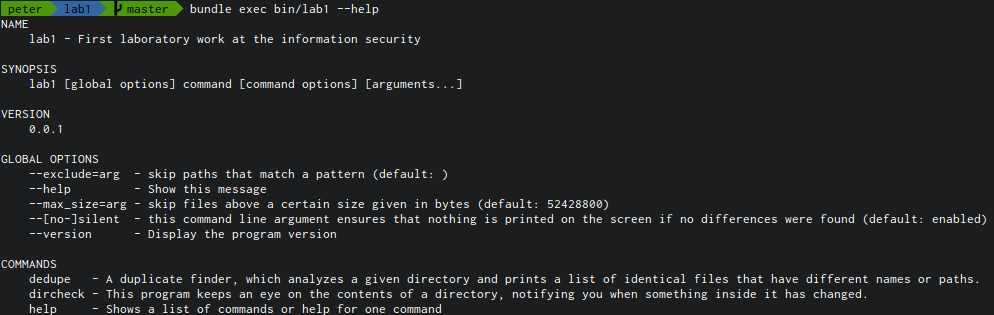
\includegraphics[width=1.0\textwidth]{help}
      % \\ Client menu
    \end{center}
  \end{minipage}

  \newpage

  \subsection{Duplication example}

   \begin{lstlisting}
    # Reopen File Class
	class File
	  def each_chunk(chunk_size=MEGABYTE)
	    yield read(chunk_size) until eof?
	  end
	end

	class DupFile
	  attr_reader :hash

	  def initialize args
	    @path = args[:path]
	    @max_size = args[:max_size]
	    @exclude = args[:exclude]
	    @hash = {}

	    calculate_size
	  end

	  def list_all_files
	    hash.inject([]) do |res, (path, info)|
	      res << "#{path} : [#{info[:size]} bytes]  [#{info[:hash]}]"
	    end.join "\n"
	  end

	  def list_same_files
	    same_files.inject([]) do |res, (hash, paths)|
	      res << "#{hash}"
	      paths.each {|path| res << path }
	      res
	    end.join "\n"
	  end

	  def same_files
	    hash_contents.group_by{|_, info| info[:hash] }
	            .each {|_, v| v.map! {|h| h.first } }
	            .select {|_, v| v.size > 1 }
	  end

	  private

	  def calculate_size
	    Dir.glob("#{@path}/**/*")
	          .reject { |file| File.directory? file }
	          .reject { |file| unwanted_paterns(file) }
	          .each  { |file| @hash[file] = {size: File.size?(file) } }
	  end

	  def filter_size
	    hash.select {|key, value| value[:size] < @max_size }
	  end

	  def hash_contents
	    filter_size.each { |path, info| @hash[path][:hash] = digest_file path }
	  end

	  def unwanted_paterns str
	   @exclude.gsub("*", "\w*").split(" ").any? { |regx| str =~ /#{regx}/ }
	  end

	  def digest_file filename
	    # Digest::SHA256.file(filename).hexdigest
	    open(filename, "rb") do |f|
	      sha256 = Digest::SHA256.new
	      f.each_chunk() {|chunk|  sha256 << chunk }
	      sha256.hexdigest
	    end
	  end

	end
   \end{lstlisting}

  \vspace{0.5cm}

  \begin{minipage}[b]{1.0\linewidth}
    \begin{center}
      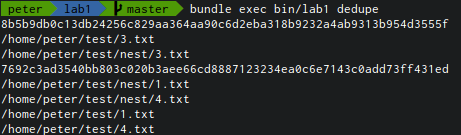
\includegraphics[width=0.5\textwidth]{dedupe1}
      % \\ Client menu
    \end{center}
  \end{minipage}

  \subsection{Modified in system}

   \begin{lstlisting}
	class DirCheck
	  attr_reader :hash

	  def initialize args
	    @path = args[:path]
	    @max_size = args[:max_size]
	    @exclude = args[:exclude]
	    @db = args[:db]
	    @rows = @db.execute( "select * from hash_table" )
	    @hash = {}
	    @result ={created: [],  deleted: [], modified: [] }
	    initiate_hash
	  end

	  # initiate hash form {path => size}
	  def initiate_hash
	    Dir.glob("#{@path}/**/*")
	          .reject { |file| File.directory? file }
	          .reject { |file| unwanted_paterns(file) }
	          .each  { |file| @hash[file] = {size: File.size?(file) } }
	  end

	  def check_contents
	    @rows.size > 1 ? search_change : fill_table
	  end

	  def show_result
	    check_contents
	    result = @result.inject([]) do |res, (status, paths)|
	      paths.each { |path| res << "#{path} (#{status})" }
	      res
	    end.join "\n"
	    refresh_table
	    result
	  end
	  def refresh_table
	    @db.execute('DELETE FROM hash_table')
	    fill_table
	  end

	  def search_change
	    check_new_files
	    check_modified_files
	  end

	  def check_new_files
	    current, old = @hash.keys, @rows.map(&:first)
	    @result[:deleted] =  old - current
	    @result[:created] = current - old
	  end

	  def check_modified_files
	    @rows.each do |db_path, db_hash, db_size|
	      if @hash.has_key?(db_path)
	        @result[:modified] << db_path if digest_file(db_path) != db_hash
	      end
	    end
	  end

	  # generate new content table
	  def fill_table
	    hash_contents.each do |path, info|
	      @db.execute("insert into hash_table values ( ?, ?,  ?)", [path, info[:hash], info[:size]])
	    end
	  end

	  def filter_size
	    hash.select {|key, value| value[:size] < @max_size }
	  end

	  # hash all files
	  def hash_contents
	    filter_size.each { |path, info|  @hash[path][:hash] = digest_file(path) }
	  end

	  def unwanted_paterns str
	   @exclude.gsub("*", "\w*").split(" ").any? { |regx| str =~ /#{regx}/ }
	  end

	  def digest_file filename
	    # Digest::SHA256.file(filename).hexdigest
	    open(filename, "rb") do |f|
	      sha256 = Digest::SHA256.new
	      f.each_chunk() {|chunk|  sha256 << chunk }
	      sha256.hexdigest
	    end
	  end

	end
   \end{lstlisting}

  \vspace{0.5cm}

  \begin{minipage}[b]{1.0\linewidth}
    \begin{center}
      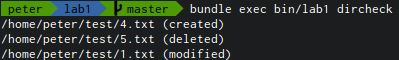
\includegraphics[width=0.4\textwidth]{dircheck1}
      % \\ Client menu
    \end{center}
  \end{minipage}


  \begin{enumerate}
  	\item Start the scheduler
  	\item Create the class responsilbe for logic
  	\item Initiate a dictionary with path and size of file
  	\item Filter by given options
  	\item Check the database if is empty introduce the data to it
  	\item If database is not empty check each file wtih current state.
  	\item And create a result based on hash comparision of them.
  \end{enumerate}


 \section{Conclussion}

	After making this laboratory work I learn about different purposes of hashing algorithms. Hash functions are related to
	(and often confused with) checksums, check digits, fingerprints, randomization functions, error-correcting codes, and ciphers,
	usually applied to detect duplicated records in a large files (similar DNA sequence) and allows one to easily verify that some
	input data matches a stored hash value. If we compare some of hash algorithms like MD5, SHA1 or SHA512 they will not improve the security of the construction so much. Computing a SHA256 or SHA512 hash is very fast. An attacker with common hardware could still try tens of millions of hashes per second. Good password hashing functions include a work factor to slow down attackers.







\end{document}

